\documentclass{article}

% Recommended, but optional, packages for figures and better typesetting:
\usepackage{microtype}
\usepackage{graphicx}
\usepackage{subfigure}
\usepackage{booktabs} % for professional tables
\usepackage{xcolor}

% hyperref makes hyperlinks in the resulting PDF.
% If your build breaks (sometimes temporarily if a hyperlink spans a page)
% please comment out the following usepackage line and replace
% \usepackage{classproject} with \usepackage[nohyperref]{classproject2025} above.
\usepackage{hyperref}


% Attempt to make hyperref and algorithmic work together better:
\newcommand{\theHalgorithm}{\arabic{algorithm}}
\newcommand{\instructions}[1]{\textcolor{blue}{#1}}

\usepackage[accepted]{classproject}
\setcitestyle{numbers,comma}

% For theorems and such
\usepackage{amsmath}
\usepackage{amssymb}
\usepackage{mathtools}
\usepackage{amsthm}

% if you use cleveref..
% \usepackage[capitalize,noabbrev]{cleveref}

%%%%%%%%%%%%%%%%%%%%%%%%%%%%%%%%
% THEOREMS
%%%%%%%%%%%%%%%%%%%%%%%%%%%%%%%%
\theoremstyle{plain}
\newtheorem{theorem}{Theorem}[section]
\newtheorem{proposition}[theorem]{Proposition}
\newtheorem{lemma}[theorem]{Lemma}
\newtheorem{corollary}[theorem]{Corollary}
\theoremstyle{definition}
\newtheorem{definition}[theorem]{Definition}
\newtheorem{assumption}[theorem]{Assumption}
\theoremstyle{remark}
\newtheorem{remark}[theorem]{Remark}

% Todonotes is useful during development; simply uncomment the next line
%    and comment out the line below the next line to turn off comments
%\usepackage[disable,textsize=tiny]{todonotes}
\usepackage[textsize=tiny]{todonotes}


% The \classprojecttitle you define below is probably too long as a header.
% Therefore, a short form for the running title is supplied here:
\classprojecttitlerunning{ECE 584 Class Project Template}

\begin{document}

\twocolumn[
\classprojecttitle{ECE 584 Class Project Final Report Template}

% List of affiliations: The first argument should be a (short)
% identifier you will use later to specify author affiliations
% Academic affiliations should list Department, University, City, Region, Country
% Industry affiliations should list Company, City, Region, Country

% You can specify symbols, otherwise they are numbered in order.
% Ideally, you should not use this facility. Affiliations will be numbered
% in order of appearance and this is the preferred way.
\classprojectsetsymbol{equal}{*}

\begin{classprojectauthorlist}
\classprojectauthor{Firstname1 Lastname1}{equal}
\classprojectauthor{Firstname2 Lastname2}{equal}
%\classprojectauthor{}{sch}
%\classprojectauthor{}{sch}
\end{classprojectauthorlist}

\classprojectcorrespondingauthor{Firstname1 Lastname1}{first1.last1@illinois.edu}
\classprojectcorrespondingauthor{Firstname2 Lastname2}{first2.last2@illinois.edu}

% You may provide any keywords that you
% find helpful for describing your paper; these are used to populate
% the "keywords" metadata in the PDF but will not be shown in the document
\classprojectkeywords{Machine Learning, Formal Verification (replace with yours)}

\vskip 0.3in
]

% this must go after the closing bracket ] following \twocolumn[ ...

% This command actually creates the footnote in the first column
% listing the affiliations and the copyright notice.
% The command takes one argument, which is text to display at the start of the footnote.
% The \classprojectEqualContribution command is standard text for equal contribution.
% Remove it (just {}) if you do not need this facility.

%\printAffiliationsAndNotice{}  % leave blank if no need to mention equal contribution
\printAffiliationsAndNotice{\classprojectEqualContribution} % otherwise use the standard text.

\begin{abstract}
Balancing an inverted single and double pendulum system on a cart is a classical problem in the field of controls and cyber physical systems. Single and double pendulums are examples of non-linear systems, and the double pendulum specifically is a chaotic system which is more difficult to control. While the control of these systems has been thoroughly studied, the verification of such cyberphysical nonlinear systems is an ongoing field of research, with single and double inverted pendulum controllers being common benchmarks in this area. In this paper, we examine Linear Quadratic Regulator controllers for single and double inverted pendulum systems and implement these controllers in the reachability analysis tool Flow* \cite{FlowStar}. We then formulate strategies to verify the stability of these controllers using Flow*. We present a straightforward method of completely verifying the single inverted pendulum controller for an initial set, as well as a method for verifying the double inverted pendulum controller. We present our verification results for both the single and double inverted pendulum controllers, and we end with a discussion on future directions.
\end{abstract}

\section{Introduction \instructions{(1 page)}}
\label{sec:intro}
The study of nonlinear cyberphysical systems is important due to the place they have in the real world. Cyberphysical systems become increasingly relevant in our lives, from autopilot controls to self-driving cars. The control of cyberphysical systems is an ongoing field of study in its own right, but the verification of such controllers is an area that still has a lot of work to be done. A couple of classic controls examples are the single inverted pendulum and double inverted pendulum cart controllers, which we aim to implement and verify using the tool Flow*. In doing so, we will build a greater understanding of strategies on how to verify nonlinear cyberphysical systems.

\paragraph{Background} 
\paragraph{Single Inverted Pendulum Controller}
\begin{figure}[H]
    \centering
    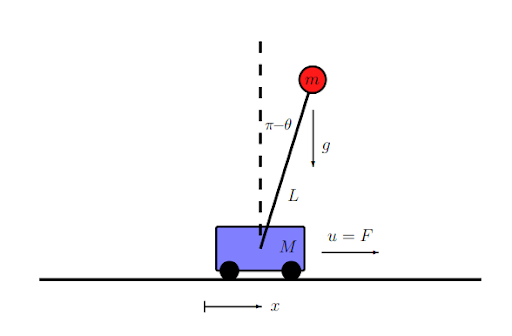
\includegraphics[scale=0.35]{image_dump/SIPC.png}
    \caption{Diagram of SIPC System}
    \label{fig:SIPC}
\end{figure}
The Single Inverted Pendulum Controller (SIPC) system we will be using is depicted above \cite{BruntonSIPC}. The state space consists of four variables: $x, v, \theta, \omega$, where $x$ and $v$ are the position and velocity of the cart, $\theta$ is the angle of the pendulum arm from the vertical position, and $omega$ is the angular velocity of the pendulum arm. There are also a number of variables we define, such as $M = 1.0$ for cart mass, $m = 0.1$ for mass of the end of the pendulum, $L = 0.5$ for length of the pendulum arm, $g = 9.81$ for the force of gravity, and $\delta = 1$ for the damping coefficient. The state space is governed by the following dynamic equations \cite{BruntonSIPC}:

\begin{equation}
    \label{SIPC_ODE}
    \begin{split}
        \dot{x} &= v \\
        \dot{v} &= \frac{\splitfrac{-m^2L^2g\cos(\theta)\sin(\theta)+mL^2\omega^2(mL\omega^2\sin(\theta)-\delta v)}{+mL^2u}}{mL^2(M+m(1-\cos(\theta)^2))} \\
        \dot{\theta} &= \omega \\
        \dot{\omega} &= \frac{\splitfrac{(m+M)mgL\sin(\theta)-mL\cos(\theta)(mL\omega^2\sin(\theta)-\delta v)}{+mL\cos(\theta)u}}{mL^2(M+m(1-\cos(\theta)^2))}
    \end{split}
\end{equation}

The system also includes an input variable $u$, which will be an input force applied horizontally to the cart. This will be driven by a controller, which will be touched upon later.

\paragraph{Double Inverted Pendulum Controller}
\begin{figure}[H]
    \centering
    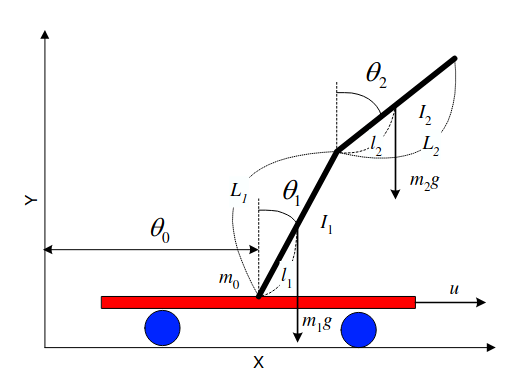
\includegraphics[scale=0.35]{image_dump/DIPC.png}
    \caption{Diagram of DIPC System}
    \label{fig:DIPC}
\end{figure}
The Double Inverted Pendulum Controller (DIPC) system we’ll be using is shown above \cite{DIPCShort,DIPCLong}. This system has a state space that consists of six variables, shown here as $(\theta_0, \theta_1, \theta_2, \dot{\theta_0}, \dot{\theta_1}, \dot{\theta_2})$. $\theta_0$ and $\dot{\theta_0}$ are the position and velocity of the cart, $\theta_1$ and $\dot{\theta_1}$ are the angle from vertical and angular velocity of the lower arm of the double pendulum, and $\theta_2$ and $\dot{\theta_2}$ are the angle from vertical and angular velocity of the upper arm of the double pendulum. User-defined variables include $m_0 = 1.5$ for the mass of the cart, $m_1 = m_2 = 0.5$ for the masses of the lower and upper arm, $L_1 = L_2 = 0.5$ for the lengths of the lower and upper arms, and $g = 9.8$ for gravitational acceleration. The image also shows variables $l_1$ and $l_2$ for the length from base of the center of gravity, and $I_1$ and $I_2$ for the moments of inertia for the two arms. To simplify the system though, it is assumed that the center of gravity is at the midpoint of each arm, so these variables don’t need to be defined.

The equations of motion \cite{DIPCShort} for this system can be written in a matrix form:
\begin{gather*}
    \textbf{D}(\theta)\ddot{\theta}+\textbf{C}(\theta,\dot{\theta})\dot{\theta}+\textbf{G}(\theta)=\textbf{H}u
\end{gather*}
where
\begin{equation}
    \label{DIPC_mat}
    \begin{split}
        &\textbf{D}(\theta)=\begin{pmatrix}
            d_1 & d_2\cos(\theta_1) & d_3\cos(\theta_2) \\
            d_2\cos(\theta_1) & d_4 & d_5\cos(\theta_1-\theta_2) \\
            d_3\cos(\theta_2) & d_5\cos(\theta_1-\theta_2) & d_6
        \end{pmatrix} \\
        &\textbf{C}(\theta,\dot{\theta})=\begin{pmatrix}
            0 & -d_2\sin(\theta_1)\dot{\theta_1} & -d_3\sin(\theta_2)\dot{\theta_2} \\
            0 & 0 & d_5\sin(\theta_1-\theta_2)\dot{\theta_2} \\
            0 & -d_5\sin(\theta_1-\theta_2)\dot{\theta_1} & 0
        \end{pmatrix} \\
        &\textbf{G}(\theta)=\begin{pmatrix}
            0 \\
            -f_1\sin(\theta_1) \\
            -f_2\sin(\theta_2)
        \end{pmatrix} \\
        &\textbf{H}=\begin{pmatrix}
            1 & 0 & 0
        \end{pmatrix}^T
    \end{split}
\end{equation}
The coefficients in these matrices are defined as:
\begin{gather*}
    \begin{aligned}
        &d_1 = m_0 + m_1 + m_2 \\
        &d_2 = (\frac{1}{2}m_1 + m_2)L_1 \\
        &d_3 = \frac{1}{2}m_2L_2 \\
        &d_4 = (\frac{1}{3}m_1 + m_2)L_1^2 \\
        &d_5 = \frac{1}{2}m_2L_1L_2 \\
        &d_6 = \frac{1}{3}m_2L_2^2 \\
        &f_1 = (\frac{1}{2}m_1 + m_2)L_1g \\
        &f_2 = \frac{1}{2}m_2L_2g
    \end{aligned}
\end{gather*}
From this, we can derive the state space dynamic equations:
\begin{equation}
    \label{DIPC_ODE}
    \dot{\textbf{x}} = \begin{pmatrix}
        \textbf{0} & \textbf{I} \\
        \textbf{0} & -\textbf{D}^{-1}\textbf{C}
    \end{pmatrix}\textbf{x} + \begin{pmatrix}
        \textbf{0} \\
        -\textbf{D}^{-1}\textbf{G}
    \end{pmatrix} + \begin{pmatrix}
        \textbf{0} \\
        \textbf{D}^{-1}\textbf{H}
    \end{pmatrix}u
\end{equation}
Again, this system also includes an input variable [u], which is the force applied horizontally to the cart by the controller.

\paragraph{Linear Quadratic Regulator}
The remaining question is how to design an optimal controller for these systems. One technique is centered around minimizing a cost function:
\begin{gather*}
    J_t=\sum_{k=t}^{t_{final}}L_k(\textbf{x}_k, \textbf{u}_k)
\end{gather*}
This represents the total accumulated cost for every state $\textbf{x}_k$ and control $\textbf{u}_k$ from time $t$ to $t_{final}$. $L_k$ in this case corresponds to Linear Quadratic cost:
\begin{equation}
    \label{LQR_cost}
    L_k(\textbf{x}_k,\textbf{u}_k) = \textbf{x}_k^T\textbf{Qx}_k+\textbf{u}_k^T\textbf{Ru}_k
\end{equation}
Here, the \textbf{Q} matrix represents the cost of deviation from the desired state, and the \textbf{R} matrix represents the cost of controller input. Both are user-defined. The dynamics equations for SIPC and DIPC can then be linearized around \textbf{x}=\textbf{0} as such:
\begin{equation}
    \label{LQR_lin}
    \dot{\textbf{x}}=\textbf{Ax}+\textbf{B}u
\end{equation}
To implement digital control, matrices A and B are approximately discretized into $\boldsymbol\Phi\approx e^{\textbf{A}\Delta t}$ and $\boldsymbol\Gamma\approx\textbf{B}\Delta t$. Optimal digital LQR control is then given by:
\begin{gather*}
    u_k = -\textbf{R}^{-1}\boldsymbol\Gamma^T\textbf{Px}_k\equiv-\textbf{Kx}_k
\end{gather*}
The \textbf{P} matrix is found by solving the discrete-time algebraic Riccati equation:
\begin{gather*}
    \boldsymbol\Phi^T[\textbf{P} - \textbf{P}\boldsymbol\Gamma(\textbf{R}+\boldsymbol\Gamma^T\textbf{P}\boldsymbol\Gamma)^{-1}\boldsymbol\Gamma^T\textbf{P}]\boldsymbol\Phi-\textbf{P}+\textbf{Q}=\textbf{0}
\end{gather*}

\paragraph{The problem.} 
\instructions{Clearly state the problem you are trying to solve. 
Important concepts in the problem statement should be defined before they are used. For example, if Graph Neural Network (GNN) or Scan lines are used in the problem statement, then those should be defined in the background paragraph.
You are encouraged to  use mathematical notations to define the problem precisely and succinctly as long as the notations are defined. 
}


\paragraph{State of the art.}
\instructions{What are the existing solutions to this problem? What are their limitations? Why is there a need for a new solution? A more detailed literature review will go in the related work section.} 

\paragraph{Your approach.}
\instructions{What is your proposed solution to the problem? How is it different from the existing solutions?}

\paragraph{Contributions}
\instructions{Summary of key contributions in this work.}


\section{Related work \instructions{(1/2 page)}}
\label{sec:related}
\instructions{Discuss the existing work in this area. What are the key contributions of previous studies? How does your work relate to or differ from these prior efforts?
You can cite papers and books using~\cite{BruntonSIPC,FlowStar,DIPCLong,DIPCShort} and include the references in the final.bib file.}

\section{Methodology \instructions{(2-3 pages)}}
\label{sec:method}
\paragraph{SIPC Implementation}
Implementing the SIPC system in Flow* is fairly straightforward. Flow* provides the functions and classes necessary to both incorporate the ODEs and the control law of the system and build a testing routine in C++. The first step is to create a Flow* Variables object and to define the necessary variables for the system. This includes both the state space variables and the input variables. For SPIC, we have four state space variables and one input variable, assigned as such:
\begin{figure}[H]
    \centering
    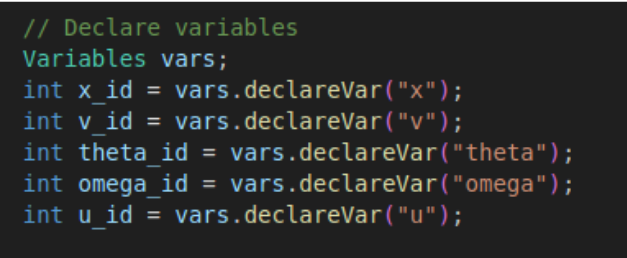
\includegraphics[scale=0.35]{image_dump/SIPC_vars.png}
    \caption{Declaring variables for SIPC}
    \label{fig:s_vars}
\end{figure}




\section{Results \instructions{(2-3 pages)}}
\label{results}

\paragraph{Benchmarks and models.}
\instructions{What benchmarks and models are used to evaluate your method?}

\paragraph{Evaluation metrics.}
\instructions{What metrics are used to evaluate the performance of your method?}

\paragraph{Results tables/graphs.}
\instructions{Present the results of your experiments using tables and graphs. You are encouraged to organize the tables according to the main lessons you want to convey.}

\paragraph{Code.}
\instructions{Provide links to your code or github repositories. Save your code and scripts in an organized fashion so that the results presented here can be replicated.}

\bibliographystyle{plain}
\bibliography{final}
\end{document}
